\chapter{Hidden Markov Models}
\section{Introduction}
The HMM is based on the Markov chain assumption. A Markov chain is a model
that tells us something about the probabilities of sequences of random variables,
states, each of which can take on values from some set. These sets can be words, or
tags, or symbols representing anything, like the weather.

There are two important assumptions:
\begin{itemize}
	\item Markov assumption
	\item Output independence: $p(x_i|z_1,\dots,z_i,\dots,z_T,x_1,\dots,x_i,\dots,x_T) = p(x_i|z_i)$
\end{itemize}

\subsection{Conditional Independence}
If two events $A$ and $B$ are \textbf{conditionally independent} given an event $C$ then,
\begin{itemize}
	\item $P(A\cap B|C) = P(A|C)P(B|C)$. 
	\item $P(A|B,C) = P(A|C)$
\end{itemize}

\subsection{Notation}

\begin{itemize}
	\item $X = (x_i, x_2,\dots, x_T)$
	% \item $x_i\in\{c_1,...,c_m\}$
	\item Initial state probabilities: $p(z_1) \sim \textrm{Multinomial}(\pi_1,...,\pi_k)$, need to learn $\pi$
	\item Transition probability:
	$$p(z_t|z_{t-1}=i)\sim \textrm{Multinomial}(a_{i,1},...,a_{i,k})$$
	, where $a_{i,j} = p(z_t=j|z_{t-1}=i)$ and $i$ and $j$ denote clusters or states, respectively.
	\item Emission probability:
	$$p(x_t|z_{t}=i)\sim \textrm{Multinomial}(b_{i,1},...,b_{i,m})$$
	, where $b_{i,j} = p(x_t=j|z_{t}=i)$
\end{itemize}


\section{Bayesian Network}
\subsection{Bayes Ball}

\begin{figure}[h!]
	\centering
	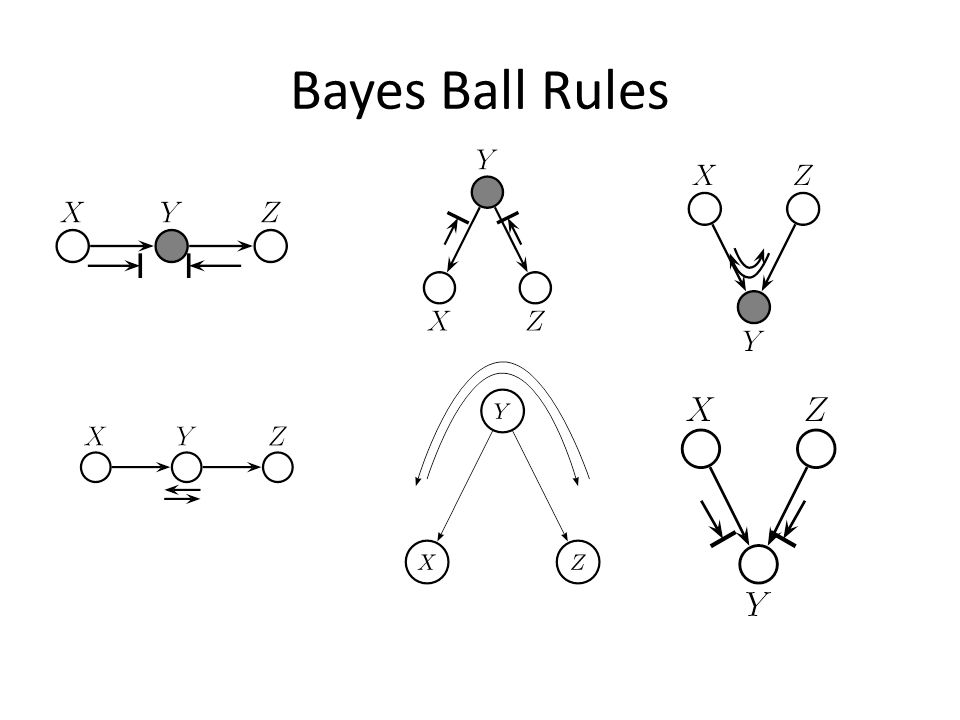
\includegraphics[scale=0.3]{./images/hmm/bayes.jpg}
	\caption{Bayes ball}
	\label{fig:bayes}
\end{figure}

\begin{itemize}
	\item Cascading: $P(Z|Y,X) = P(Z|Y)$. The information of $Y$ decouples $X$ and $Z$.
	\item Common parent: $P(X,Z|Y) = P(X|Y)P(Z|Y)$. The information of $Y$ decouples $X$ and $Z$.
	\item V-Structure (common child): Unlike the above two cases, the information of $Y$ couples $X$ and $Z$.
		$$P(X,Y,Z) = P(X)P(Y)P(Y|X,Z).$$
\end{itemize}

\subsection{Potential Function}
Potential function is a function which is not a probability function, but it can become a probability function by normalizing it. 
$$P(A,B,C,D) = P(A|B)P(B|C)P(C|D)P(D)$$

\begin{figure}[h]
	\centering
	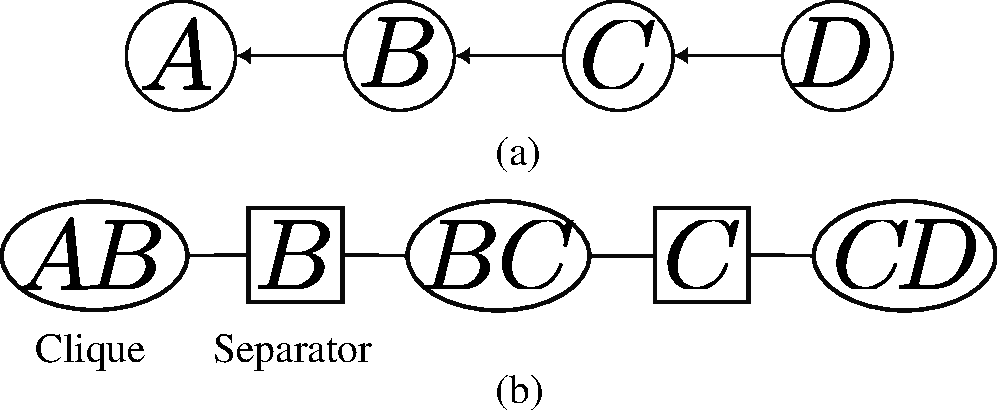
\includegraphics[scale=0.5]{./images/hmm/cascade.pdf}
\end{figure}

\begin{itemize}
	\item Cliques: $\Psi(a,b), \Psi(b,c), \Psi(c,d)$
	\item Separators $\phi(b), \phi(c)$
\end{itemize}
Given a clique tree with cliques and separators, the joint probability distribution is defined as follows:
% By using potential functions, we can express the joint probability as
\begin{align*}
	P(A,B,C,D) &= P(U) = \frac{\prod_N \Psi(N)}{\prod_L\phi(L)}= \frac{ \Psi(a,b)\Psi(b,c)\Psi(c,d)}{\phi(b)\phi(c)}\\
\end{align*}
An effect of an observation propagates through the clique graph $\to$ \textbf{Belief propagation}. How to propagate the belief? \textbf{Absorption rule}!

Let's say we have some new observations about $A$, then it affects the clique $\Psi(a,b)$. The updated clique is now $\Psi^*(a,b)$. Similarly, $\phi^*(b) = \sum_A\Psi^*(a,b)$. Subsequently, $\Psi^*(b,c) = \Psi^(b,c)\frac{\phi^*(b)}{\phi(b)}$.

\newpage
\section{Hidden Markov Models}
\label{sec:hmm}

\begin{figure}[h]
	\begin{center}
		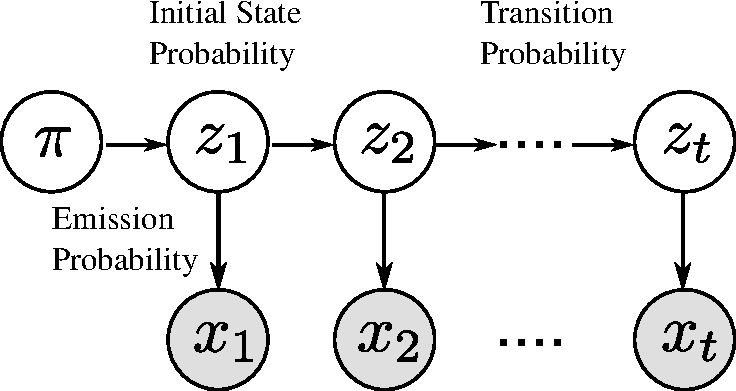
\includegraphics[scale=0.7]{./images/hmm/hmm_figure.pdf}
	\end{center}
	\caption{HMM Structure}
	\label{fig:HMM}
\end{figure}

The observation can be discrete or continuous. If the latent factors are continuous, then HMM is often referred as \textbf{Kalman filter}. 

\begin{itemize}
	\item Initial state probability: $P(z_1)\sim \textrm{Mult}(\pi_1, \dots, \pi_k)$
	\item Transition probability: $P(z_t|z^i_{t-1}=1)\sim \textrm{Mult}(a_{i,1}, \dots, a_{i,k})$, \\ where $P(z_t^j=1|z_{t-1}^i=1) = a_{i,j}$
	\item Emission probability: $P(x_t|z_t^i=1)\sim \textrm{Mult}(b_{i,1}, \dots, b_{i,m})\sim f(x_t|\theta_i)$,\\ where $P(x_t^j=1|z_{t}^i=1) = b_{i,j}$. The probability of observing $x_j$ at the  $i$-th cluster. 
\end{itemize}
Note that $i$ and $j$ are indices of clusters. 

There are three main problems in HMM:
\begin{enumerate}
	\item Evaluation Questions (likelihood): %Forward algorithm
	\begin{itemize}
		\item Given $\boldsymbol{\pi}\mathbf{, a, b}, X$
		\item Find $p(X|M, \boldsymbol{\pi}\mathbf{, a, b})$
		\item How much are $X$ likely to be observed by a model $M$?
	\end{itemize}
	
	\item Decoding Questions:
	\begin{itemize}
		\item Given $\boldsymbol{\pi}\mathbf{, a, b}, X$
		\item Find $\argmax_Z p(Z|X, M, \boldsymbol{\pi}\mathbf{, a, b})$
		\item What is the most probable sequence of $Z$ (latent states)? 
	\end{itemize}
	
	\item Learning Questions: Forward-Backward (Baum-Welch)
	\begin{itemize}
		\item Given $X$
		\item Find $\argmax_{\boldsymbol{\pi}\mathbf{, a, b}} p(X|M, \boldsymbol{\pi}\mathbf{, a, b})$
		\item What would be the optimal model parameters? 
	\end{itemize}
\end{enumerate}

% For a given hidden state, we can easily compute the output likelihood.
